\documentclass[11pt]{article}
\usepackage[margin=1in]{geometry}
\usepackage{amsmath,amssymb,amsthm,booktabs,enumitem,xcolor,graphicx}
\setlist[itemize]{label=$\bullet$}
\usepackage[hidelinks,pdftitle={The Neutrinos at the Wall},pdfauthor={Jeromie Beasley}]{hyperref}
\newtheorem{theorem}{Theorem}\newtheorem{proposition}[theorem]{Proposition}\newtheorem{lemma}[theorem]{Lemma}
\theoremstyle{definition}\newtheorem{hypothesis}{Hypothesis}\newtheorem{prediction}{Prediction}
\theoremstyle{remark}\newtheorem{remark}[theorem]{Remark}
\newcommand{\grade}[1]{\textsf{\small[#1]}}
\setlength{\parskip}{0.3em}
\title{The Neutrinos at the Wall:\\ Mass, Decoupling, and a Record That Passes Through the Fold}
\author{Jeromie Beasley}
\date{15 November 2026}
\begin{document}
\maketitle

\noindent\emph{AI-assisted. The ideas and research direction are the author's. AI tools (Claude, Anthropic) were used for literature search, computation, drafting and typesetting. Every number not taken from the author's archived runs or from a cited source is computed by the scripts \texttt{wall\_checks.py} and \texttt{fig\_wall.py}, or by the experiment scripts of the pocket record~\cite{Pocket}, all described in Appendix~C. Grades: \grade{derived} proved here or in the cited paper of the author; \grade{measured} computed from runs; \grade{reading} an interpretation; \grade{H} a hypothesis with a stated test.}

\begin{abstract}
One wall organises this paper. In the author's link coordinate $\Gamma=\tanh(\tfrac12\ln z)$, two equal perpendicular steps of ratio $z$ have a commutator of trace $2-4\sinh^4(\tfrac12\ln z)$. That commutator turns parabolic, the boundary between turning and passing, at exactly $z=3+2\sqrt2$, $\Gamma^2=\tfrac12$. Seen from the rim, where every point is a direction of light, it is the step that first sends every direction outside the opposite $45^\circ$ cap into its own.

The neutrinos sit on this wall twice. First, in their masses. With the lightest neutrino massless, the current oscillation data give $m_3/m_2=5.807\pm0.052$, which is $0.41\sigma$ from $3+2\sqrt2=5.8284$ (NuFIT~6.0 alone: $5.8165\pm0.079$, $0.15\sigma$). The relation is Alikhanov's; what is new here is its place as the wall. On the wall's own picture, the square of two such steps is a turn whose centre sits near the rim, while every charged step's square is a run to the rim. Every charged-fermion generation step lies past the wall, $\Gamma$ from $0.89$ to $0.997$. Taking the neutrino step to lie on the wall exactly fixes:
\begin{itemize}[nosep]
\item normal ordering;
\item $m_2=8.65$ and $m_3=50.44$\,meV;
\item $\Sigma m_\nu=59.1$\,meV;
\item $\Delta m^2_{31}/\Delta m^2_{21}=(1+\sqrt2)^4=33.97$, against $33.72$ measured ($33.83$ on NuFIT~6.0);
\item a lightest mass below about $1.5$\,meV;
\item $m_\beta=8.85$\,meV and, at $m_1=0$, $m_{\beta\beta}\in[1.5,3.7]$\,meV.
\end{itemize}

Second, in how the neutrinos let go of the plasma. The isotropic sector of their transport operator has a kept mode only while the collision rate exceeds $\kappa=2k/\pi$. There its non-orthogonality $4\phi^2/\sin^22\phi$ diverges and the mode merges into free streaming. All the non-normality sits on the density--flux link, with weight equal to the sound speed. The neutrinos are the first species to cross this wall, at about $1$\,MeV, across an electron--positron layer that later heats only the light.

A record carried across this wall is physical. In S.~McCormick's general-relativistic collapse code, two neutrino states identical in density, flux, stress and every metric quantity, differing only in hidden angular structure planted at decoupling, have black-hole thresholds up to $5.5\times10^{-3}$ apart. In a Gaussian universe, at the planted amplitude, that changes the number of black holes near $4\times10^4\,M_\odot$ by 5--47\%, with a sign set by the record's orientation; a record of random orientation still raises it, by up to 8\%. The planted amplitude is engineered, half of each cell's positivity margin, and only that amplitude was run.

Finally, the author's fold theorem, proved for four-body shape space and the static base of a horizon, has a counterpart in the radiation era. Cosmic time is the even observable and the conformal scale factor the signed one, so the apparent beginning is a fold at finite distance, and the path continues through it to the mirror. What crosses depends on how hot the passage is. A hot rebirth erases any record that collisions act on directly: an angular record keeps $10^{-4}$ of itself from $3$\,MeV and $10^{-145}$ from $10$\,MeV. Through a cold fold a few per cent returns, with no even/odd rule. What no collision can erase is a conserved charge. For the neutrinos that is the lepton asymmetry, the author's offset $\mu$: collisions keep each flavour's number, oscillations keep the total, and the electron sea's thermal potential holds the flavour split while it is hot, though full three-flavour treatments share the asymmetry among the flavours before nucleosynthesis. A universe that recurs through such folds can hand the neutrinos a common chemical potential at decoupling, which helium and $N_{\rm eff}$ measure.

The paper states each prediction with the experiment that can refute it. It credits the prior work it meets: Alikhanov for the mass relation, Boyle, Finn and Turok for the mirror continuation and a massless lightest neutrino, McCormick for the collapse code and the free-streaming effect, and Dolgov and collaborators for flavour equilibration of neutrino asymmetries.
\end{abstract}

\tableofcontents

\section{The claim}\label{sec:claim}

A wall, in the author's work, is not where something is stored. It is where a memory exerts force: what arrives across it is written in, and nothing written inside can write back~\cite{BH}. The author has met such walls in four-body shape space, in the static base of a horizon, at the innermost stable orbit of a black hole, in the Sun's dynamo, and at an optical threshold~\cite{BH,Light,Suns}. At each of them two things survive exactly, whatever happens to the individual eigenvectors: the contour's ledger and the orientation. \emph{The contour keeps the ledger; the orientation keeps the trace}~\cite{BH}.

This paper's claim is that the neutrinos are the particles at such a wall, in three ways that can be checked:
\begin{enumerate}[nosep]
\item their heaviest mass step lies on the wall $\Gamma^2=\tfrac12$ where a pair of equal perpendicular steps turns parabolic (Section~\ref{sec:masses});
\item their decoupling is the same kind of wall in motion. The kept sector of their transport loses its mode at $\kappa=2k/\pi$, and they are the first species to cross (Section~\ref{sec:letgo});
\item a record carried across it changes how many black holes form (Section~\ref{sec:bh}), and a universe that passes through a fold rather than beginning can supply a record, in the one form a hot rebirth cannot erase (Section~\ref{sec:fold}).
\end{enumerate}
Section~\ref{sec:tests} collects every prediction with the measurement that can refute it. Section~\ref{sec:notclaimed} says what is not claimed. Temperatures, the horizon mass and the expansion history used below are the standard-cosmology coordinates of McCormick's code, used as a tool; the author does not hold that the universe began in a big bang, and Section~\ref{sec:fold} is where that view enters.

\section{The wall}\label{sec:wall}

\subsection{The link coordinate}
Two books, two rates, two masses: any positive pair $d_i,d_j$ forms a link with ratio $z=d_i/d_j$, rapidity $\tfrac12\ln z$ and Smith coordinate
\begin{equation}
\Gamma=\frac{z-1}{z+1}=\tanh\big(\tfrac12\ln z\big),\qquad \frac{E^-}{E^+}=\Gamma^2 ,
\end{equation}
where $E^\mp$ are the two books of the link~\cite{VOTKP,Atlas}. Exchanging the ends negates $\Gamma$. A matched link, $z=1$, sits at the centre of the chart. The same coordinate is the reflection coefficient of a wave at a change of spectral gap, $\Gamma=\tanh(\tfrac12\ln\Delta_2/\Delta_1)$~\cite{BH}, and the neutrino transport's flux--shear link $\Gamma_{12}=(r-1)/(r+1)$~\cite{NU10}.

\subsection{Where a pair of steps turns parabolic}
\begin{theorem}[the wall of two equal perpendicular steps]\label{thm:wall}\grade{derived; Appendix A.1; checked}
Let $B_x(r)$ and $B_y(r)$ be boosts of rapidity $r$ along perpendicular axes in $SL(2,\mathbb C)$, and $K=B_xB_yB_x^{-1}B_y^{-1}$ their commutator. Then
\begin{equation}
\operatorname{tr}K=2-4\sinh^4(r/2).
\end{equation}
$K$ is elliptic (a pure turn) for $\operatorname{tr}K\in(-2,2)$, parabolic at $\operatorname{tr}K=-2$, and hyperbolic beyond. The parabolic wall is at
\begin{equation}
r_w=\ln(3+2\sqrt2)=1.762747,\qquad z_w=e^{r_w}=3+2\sqrt2=5.828427,\qquad \Gamma_w=\tanh(r_w/2)=\frac1{\sqrt2}.
\end{equation}
\end{theorem}
This is the author's BallJoins J3--J4 and atlas cards B189 and B199~\cite{TwoTrees,Atlas,SMball}. The Lean statements \texttt{line\_ratio} and \texttt{five\_inside\_seven\_outside} cover the ratio identity $(1+\Gamma)/(1-\Gamma)=z$ and the cases $z=5$ (inside) and $z=7$ (outside); the exact threshold is the algebra of Appendix A.1, checked numerically. The Lean repository was not re-run for this paper. Below $z_w$ a loop of two perpendicular steps closes as a turn: a bound orbit, a spin. Above it the loop climbs and turns: a flyby. On the wall it does neither: a Jordan block, the parabolic case. A black hole carries exactly this kind of wall at its innermost stable circular orbit, where the wobble generator of circular orbits squares to zero and gravity's effective power reaches the inverse cube, $p=2+6M/r=3$~\cite{BH}.

\paragraph{The wall seen from the balls.} The same wall has a picture in the author's ball~\cite{TwoTrees,Mixer}. Put a ball at the centre and a neighbour one step of ratio $z$ out along each of two perpendicular arms. Between the centre and each neighbour stands the face halfway, at rapidity $\tfrac12\ln z$. For two equal steps
\begin{equation}
g=\sinh^2\big(\tfrac12\ln z\big)=\frac{(z-1)^2}{4z}.
\end{equation}
\begin{proposition}[turn or run~\cite{TwoTrees}, Theorems 5.3, 5.4 and 8.4]\label{prop:turnrun}\grade{derived there; Lean BallJoins J3, J4, J7; checked, Appendix C}
If $g<1$ the two faces cross, at the angle $\arccos g$, and the square of the two steps (step $a$, step $b$, back $a$, back $b$) is a turn by $4\arccos g$ about a fixed point at
\begin{equation}
\tanh^2\frac{\rho}{2}=\frac{1-s}{1+s},\qquad s=\sqrt{1-2\Gamma^2}.
\end{equation}
Repeating it carries the centre round a ring: the walk is held. If $g>1$ the faces stand apart by $\operatorname{arccosh}g$ and the square is a run of length $4\operatorname{arccosh}g$: repeating it carries the centre to the rim. At $g=1$ the faces just touch, $s=0$, and the fixed point reaches the rim. This is the wall of Theorem~\ref{thm:wall}: $g=1$ is $\sinh(r/2)=1$. Reversing one step, or the order, reverses the sense of the turn.
\end{proposition}
The turn angle follows from Theorem~\ref{thm:wall}: the half-trace of the square is $1-2g^2=\cos(\pi-2\arccos g)$, so the turn is $2\pi-4\arccos g$, a turn of size $4\arccos g$ in the opposite sense.

\paragraph{The wall seen from the rim.} The rim of the ball is the set of light directions~\cite{Mixer2}. A step of rapidity $r$ along a unit axis $u$ moves a direction at angle $\psi$ from $u$ by the same Smith addition that composes steps,
\begin{equation}
\cos\psi'=\frac{\cos\psi+\tanh r}{1+\cos\psi\,\tanh r}=\cos\psi\oplus\tanh r ,
\end{equation}
and the face halfway to the neighbour, at rapidity $r/2$, meets the rim on the circle $\cos\psi_0=\tanh(r/2)=\Gamma$~\cite{Mixer2}.
\begin{proposition}[the wall on the rim]\label{prop:rim}\grade{derived here; checked, Appendix C}
One step of ratio $z$ sends every light direction outside the open $45^\circ$ cap about $-u$ into the closed $45^\circ$ cap about $u$ exactly when $z\ge3+2\sqrt2$. On the wall the face meets the rim on the $45^\circ$ circle itself.
\end{proposition}
\begin{proof}
$\cos\psi'$ increases with $\cos\psi$, so the worst direction is the edge of the excluded cap, $\cos\psi=-1/\sqrt2$. With $t=\tanh r$ the condition $(t-1/\sqrt2)/(1-t/\sqrt2)\ge1/\sqrt2$ reads $\tfrac32t\ge\sqrt2$, that is $t\ge2\sqrt2/3$. For $z=e^r$, $\tanh r=(z^2-1)/(z^2+1)$, and $z=3+2\sqrt2$ gives $z^2=17+12\sqrt2$ and $\tanh r=(16+12\sqrt2)/(18+12\sqrt2)=2\sqrt2/3$. On the wall $\Gamma=1/\sqrt2$, so $\psi_0=45^\circ$.
\end{proof}
This is the cap condition of the ping-pong argument for the three perpendicular steps; the author's Lean statement covers $z=7$, and the mixer checks it numerically just above the wall and fails it at $z=5$~\cite{Mixer2}. Two steps along different arms also compose into one step and a turn of the frame, the Thomas turn, with $\tan(\theta_T/2)=\Gamma_a\Gamma_b$~\cite{TwoTrees,Mixer2}. For two equal steps on the wall $\tan(\theta_T/2)=\tfrac12$, so $\cos\theta_T=\tfrac35$ exactly, $\theta_T=53.13^\circ$; the measured neutrino step gives $53.01^\circ$ \grade{computed, Appendix C}. The Thomas turn is of a frame and is not a statement about polarisation.

\subsection{Two kinds of wall, and what survives}
The author sorts walls into two kinds~\cite{BH}.
\begin{itemize}[nosep]
\item At a \emph{spectral} wall a real pair of eigenvalues turns complex along a physical path, and the Jordan block is present in every frame. Examples: the innermost stable orbit, the Sun's dynamo wave, the optical threshold.
\item At a \emph{geometric} wall, or fold, the spectrum stays real on both sides. The block belongs only to the folded chart, and the path passes through to a mirror configuration. Examples: the coplanar wall of four-body shape space, the static base of a horizon.
\end{itemize}

\begin{theorem}[the fold~\cite{BH}, Theorem 2]\label{thm:fold}\grade{derived there}
Let an even observable $X$ be the square of a signed coordinate $\lambda$, $X=\lambda^2$. A metric that is regular and even in $\lambda$ reads $ds^2=dX^2/(4c^2X)$ in $X$. Its coefficient diverges at $X=0$, while the distance to the wall is finite and the path continues to $\lambda<0$, the mirror. On four-body shape space $c=1$ and the distance from the wall to $w_3=\varepsilon$ is $\arcsin\sqrt\varepsilon$. On the Schwarzschild static base $c=\kappa$, the surface gravity.
\end{theorem}

What passes a wall of either kind is fixed by two survival principles. Both are proved in~\cite{BH}.
\begin{itemize}[nosep]
\item The Riesz projector of the colliding pair and its trace-log ledger, $\log\det(c+A_{\rm pair})$, stay exact through the wall in every frame, where single eigenprojectors diverge like $|A_{12}|/\mathrm{gap}$.
\item The orientation, the sign of $\det X$ and the analytic label of the branch, survives as a $\mathbb Z_2$ record that the even observer cannot see. Readings odd under the mirror cancel across it; even readings survive.
\end{itemize}
Compression at a wall, $X\mapsto PXP$, is ``rank compression, not destruction''~\cite{BH}.

\section{The masses at the wall}\label{sec:masses}

\subsection{Charged fermions step past the wall}
Read as links, the generation steps of the charged fermions are all hyperbolic. They lie past $z_w$, with $\Gamma$ from $0.888$ ($\mu\to\tau$, $z=16.8$) to $0.997$ ($u\to c$, $z=589$) \grade{measured, \cite{SMball}}. The charged leptons have a second structure. Koide's $Q=(m_e+m_\mu+m_\tau)/(\sqrt{m_e}+\sqrt{m_\mu}+\sqrt{m_\tau})^2$ is $0.666664463$ with the PDG $\tau$ mass $1776.93$\,MeV~\cite{PDG}, so the vector $(\sqrt{m_e},\sqrt{m_\mu},\sqrt{m_\tau})$ makes an angle with $\cos^2=1/(3Q)=0.50000165$ with $(1,1,1)$~\cite{Koide} \grade{computed, Appendix C}. In the author's atlas this is a link with \emph{balanced books}, $E^-=E^+$ (card B200)~\cite{Atlas}. It is a different condition from the wall $E^-/E^+=\tfrac12$ of card B189, and the two are not identified here \grade{reading}.

\subsection{The neutrinos' heaviest step is on the wall}
With normal ordering and $m_1=0$, the oscillation splittings fix $m_2=\sqrt{\Delta m^2_{21}}$ and $m_3=\sqrt{\Delta m^2_{31}}$. The NuFIT~6.0 central values~\cite{NuFIT} (normal ordering, the table without Super-Kamiokande atmospheric data: $\Delta m^2_{21}=(7.49\pm0.19)\times10^{-5}$, $\Delta m^2_{31}=2.534^{+0.025}_{-0.023}\times10^{-3}$\,eV$^2$) give
\begin{equation}
\frac{m_3}{m_2}=5.8165\pm0.079\quad\text{against}\quad z_w=3+2\sqrt2=5.8284,
\end{equation}
a difference of $-0.15\sigma$ \grade{computed, Appendix C}. The table with Super-Kamiokande atmospheric data, $\Delta m^2_{31}=2.513\times10^{-3}$\,eV$^2$, gives $5.792\pm0.077$, $-0.47\sigma$. Equivalently $\Delta m^2_{31}/\Delta m^2_{21}=33.83$ against $(1+\sqrt2)^4=33.97$. With the first JUNO measurement $\Delta m^2_{21}=(7.50\pm0.12)\times10^{-5}$\,eV$^2$ and NuFIT~6.1's $\Delta m^2_{31}=(2.529\pm0.021)\times10^{-3}$\,eV$^2$, the inputs Alikhanov uses and quotes~\cite{Alik}, the ratio is $33.72$ and
\begin{equation}
\frac{m_3}{m_2}=5.807\pm0.052,
\end{equation}
$-0.41\sigma$ from the wall \grade{computed, Appendix C}. The two inputs come from different fits, combined here as Alikhanov combines them. The match was found after the relation was proposed, and the wall is one of a few simple constants on the chart that could have been tried, so it is a coincidence to test, not evidence on its own. The relation $(m_3+m_2)/(m_3-m_2)=\sqrt2$ with $m_1=0$ was proposed by Alikhanov~\cite{Alik}. It is the same number. What this paper adds is its place: it is the link $\Gamma^2=\tfrac12$ of Theorem~\ref{thm:wall}.

\begin{figure}[t]\centering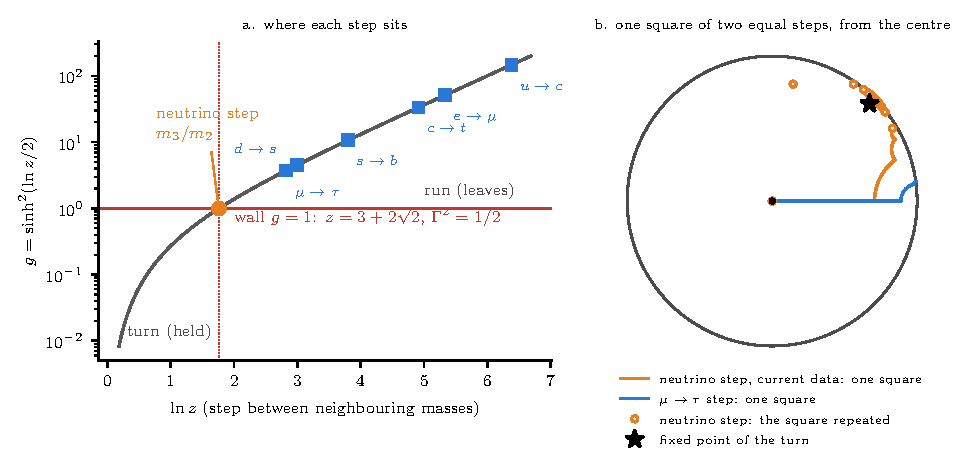
\includegraphics[width=\textwidth]{fig_wall.pdf}
\caption{The neutrino step at the wall. (a) $g=\sinh^2(\tfrac12\ln z)$ for each step between neighbouring masses. The wall $g=1$ is $z=3+2\sqrt2$; the neutrino step $m_3/m_2$ (both data sets) sits on it, every charged generation step lies past it. (b) One square of two equal steps from the centre of the ball, computed from the boost matrices. The neutrino step (current central value) closes into a turn of $23.4^\circ$ about a fixed point near the rim (star, $\tanh(\rho/2)=0.950$); the square repeated walks the ring round it (open circles). At $+1\sigma$ the same square is a short run: the data do not decide between the two. The $\mu\to\tau$ step is a run of length $7.95$ that ends at the rim. Script \texttt{fig\_wall.py}.}\label{fig:wall}\end{figure}

The charged steps pass the wall. The neutrino step sits on it, within the errors. Figure~\ref{fig:wall} shows both by Proposition~\ref{prop:turnrun}. With the measured step the square of two neutrino steps is a turn of $23.4^\circ$ (current data; $17.4^\circ$ on NuFIT~6.0) about a fixed point at $\tanh(\rho/2)=0.950$ ($0.963$): held, at the edge. The $\mu\to\tau$ step, the smallest charged step, gives a run of length $7.95$ \grade{computed, Appendix C}. The data do not decide turn against run for the neutrino step. Near $g=1$ the turn angle goes like the square root of the distance to the wall: at $-1\sigma$ the square is a turn of $43^\circ$, at $+1\sigma$ a run of length $0.49$, and a Gaussian on the current ratio puts $34\%$ of its weight on the run side ($44\%$ on NuFIT~6.0) \grade{computed, Appendix C}. What the data do say is that the neutrino step is at the wall and every charged step is far past it. Read in the ball, the neutrinos are held at the line, and every charged step runs out \grade{reading}. The neutrinos are also the particles that sit just inside the rim of the author's ball, the velocity space of one massive particle: at a common energy of 1\,MeV a $0.05$\,eV neutrino sits at ball radius $1-5\times10^{-8}$, with $1-v=1.25\times10^{-15}$ \grade{computed, Appendix C}.

Theorem~\ref{thm:wall} concerns two equal perpendicular steps; reading one mass ratio as both of them is the reading of the author's ball, where the generation step is taken along two arms at once~\cite{SMball,Mixer2}. For unequal steps the square changes at $g=\sinh h_a\sinh h_b=1$, not where either step alone crosses the wall~\cite{Mixer2}. Read as an admittance step, a single face on the wall returns exactly half, $R=T=\tfrac12$~\cite{Mixer2}.

\begin{hypothesis}[the neutrino step is the wall]\label{hyp:mass}
The neutrino mass step is exactly parabolic, $m_3/m_2=3+2\sqrt2$, with $m_1$ negligible.
\end{hypothesis}

Why the neutrinos land on the wall rather than past it is not derived here. The reading the author's work offers is this. A wall is where a memory exerts force and does not store it. The neutrinos are the species whose whole role in the universe's history is to let go first and carry the record outward (Section~\ref{sec:letgo}). A step on the wall is the step that neither binds (turns) nor escapes (climbs) \grade{reading}.

\subsection{What the hypothesis fixes}
\begin{center}\small\begin{tabular}{p{0.27\textwidth}p{0.36\textwidth}p{0.29\textwidth}}\toprule
quantity & value on the wall & status today\\\midrule
mass ordering & normal & favoured, not settled\\
lightest mass $m_1$ & $\lesssim1.5$\,meV (exact wall: $0$) & open\\
$m_2,\ m_3$ & $8.65$, $50.44$\,meV & consistent\\
$\Delta m^2_{31}/\Delta m^2_{21}$ & $(1+\sqrt2)^4=33.971$ & $33.72$ ($33.83$ NuFIT~6.0)\\
$\Delta m^2_{31}$ given $\Delta m^2_{21}$ & $2.544\times10^{-3}$\,eV$^2$ & $2.534\times10^{-3}$\\
$\Sigma m_\nu$ & $59.1$\,meV ($59.0$--$60.6$ for $m_1\le1.5$\,meV) & near cosmological bounds (model-dependent)\\
$m_\beta$ & $8.85$\,meV ($\le8.96$) & far below current direct searches\\
$m_{\beta\beta}$ (if Majorana) & $1.5$--$3.7$\,meV at $m_1=0$; $0.5$--$4.8$\,meV for $m_1\le1.5$\,meV & target for future searches\\\bottomrule\end{tabular}\end{center}
\grade{derived from Hypothesis~\ref{hyp:mass}; $m_2$, $m_3$, $m_\beta$, $m_{\beta\beta}$ and $\Delta m^2_{31}$ from NuFIT~6.0 central values, the bound on $m_1$ and the first ratio from the current inputs; Appendix C}. On the current inputs $m_2=8.66$ and $m_3=50.48$\,meV, and $\Sigma m_\nu$ is still $59.1$\,meV.

The sensitivity to $m_1$ is steep. The measured step $\sqrt{(m_1^2+\Delta m^2_{31})/(m_1^2+\Delta m^2_{21})}$ falls to $5.779$ at $m_1=1$\,meV, $5.672$ at $2$\,meV and $5.061$ at $5$\,meV. On NuFIT~6.0 the wall therefore requires $m_1$ below about $2$\,meV. On the current inputs the pull reaches $-2\sigma$ at $m_1=1.5$\,meV, so at $2\sigma$ the wall requires $m_1$ below about $1.5$\,meV. Inverted ordering gives a step near $1$, deep inside the wall.

Boyle, Finn and Turok predicted a massless lightest neutrino from an entirely different argument, CPT symmetry of the universe across what they take to be the bang~\cite{BFT,BFT2}. Section~\ref{sec:fold} meets their construction again. Here it suffices that two independent routes ask for $m_1=0$, and the present one additionally fixes the ratio of the other two.

\section{Letting go: decoupling is the same wall in motion}\label{sec:letgo}

\subsection{The cut}
For one Fourier mode $k$ the linearised neutrino intensity evolves under $L=-ik\mu-\kappa(I-P)$. Here $P$ projects onto the isotropic part, the kept sector, and $\kappa$ is the collision rate~\cite{McC,NU10}. In the Legendre basis streaming links only neighbours, with weights $c_\ell=(\ell+1)/\sqrt{(2\ell+1)(2\ell+3)}$. Collisions are diagonal.
\begin{proposition}[the cut~\cite{NU10,CE}]\grade{derived there; Lean}
$\tfrac18\lVert[L,L^*]\rVert_F^2=\sum_\ell k^2c_\ell^2(D_{\ell+1}-D_\ell)^2$. For one rate all of it sits on the density--flux link, $\kappa^2k^2/3$. The weight across the cut is $\sqrt{E_B}=\lVert PH(I-P)\rVert=k/\sqrt3$, the radiation sound speed times $k$.
\end{proposition}
The kept sector therefore moves at the sound speed, while what leaves it moves at the speed of light.

\subsection{The kept mode exists only above a wall}
The isotropic part has the exact propagator $\langle0|(s-L)^{-1}|0\rangle=g/(1-\kappa g)$, with $g=k^{-1}\arctan[k/(s+\kappa)]$~\cite{NU10}. A kept mode is a pole, $\kappa g=1$.
\begin{theorem}[the decoupling wall~\cite{NU10}; onset of Romatschke~\cite{Rom}]\label{thm:onset}\grade{derived there}
With $\phi=k/\kappa$ the kept mode is $s=k\cot\phi-\kappa$. It exists only for $\phi<\pi/2$, that is $\kappa>2k/\pi$. Its non-orthogonality, the squared ratio of its norm to its bilinear self-pairing, is
\begin{equation}
K=\frac{4\phi^2}{\sin^22\phi},
\end{equation}
equal to $1$ for a fully coupled gas and divergent at the wall, where the mode meets the branch cut of $g$ at its centre and merges into free streaming.
\end{theorem}
$K$ rises from $1.41$ at $\phi=0.5$ to $4.84$ at $\phi=1$, $69.9$ at $\phi=1.4$ and $5558$ at $\phi=1.55$ \grade{derived; Appendix C}. As the plasma cools in this setting, $\kappa/k$ falls through $2/\pi$ for each scale in turn. That is the wall in motion. Before it the gas relaxes everything but the kept sector, and hidden structure is damped. After it the gas lets go.

\subsection{The neutrinos are first, and an electron layer lies between}
The neutrinos cross this wall at a temperature of about $1$\,MeV. The photons cross their own, against the electrons, only near $0.26$\,eV. Between the two lies the electron--positron plasma. The neutrinos let go of it first. Then its annihilation near $0.5$\,MeV heats the photons and not the neutrinos~\cite{Dolgov}. The ordering is: neutrino side, electron layer, light side \grade{cited physics}. The author's own boundary work treats the laboratory version of such a layer, the electron screening cloud at a nuclear barrier~\cite{Screen}.

The neutrinos are fermions, and that fixes what their outside record can be. For a fermion pair the outside occupation $C$ has a definite offset
\begin{equation}
\tau=\log\frac{1-C}{C}=\frac{\hbar\omega}{k_BT},\qquad \Gamma=\tanh\frac{\hbar\omega}{2k_BT},
\end{equation}
for every pair phase, a point on the same Smith chart as the wall~\cite{BH,Offset}. A boson record has no ``full'' state and no such offset. Light and the neutrinos are the boson and fermion sides of one thermal record \grade{derived in~\cite{BH}; reading}. At decoupling the typical neutrino ($\hbar\omega\approx3.15\,k_BT$) sits at $\Gamma=0.918$, far out on the chart \grade{derived}. A chemical potential shifts the offset of every pair by the same amount, $\tau=(\hbar\omega-\mu)/k_BT$; in the cosmological literature this is the degeneracy $\xi=\mu/k_BT$. Section~\ref{sec:fold} shows it is the one neutrino record a hot rebirth cannot erase.

\subsection{Where the record lives}
A fluid closure keeps density, flux and stress ($\ell\le2$). The author proved that eliminating the hidden moments $\ell\ge1$ exactly gives the kept amplitude one equation,
\begin{equation}
\dot a(t)=S(t)-k^2\!\int_s^tK(t,r)\,a(r)\,dr,
\end{equation}
with the whole hidden past in one source $S$ and one memory kernel $K$~\cite{NU10}. The kept population obeys the speed limit $\dot A^2\le4E_BA(1-A)$~\cite{NU10} \grade{derived there; Lean}. Hidden structure planted while the gas is coupled is erased by $\exp[-\epsilon_{\rm dec}^n/(n\tau_s^n)]$. Planted at or after decoupling, it returns into density, flux and stress at the several-per-cent level. The readout Gramian of the hidden sector has no kernel, so every hidden direction is eventually seen. Its spectrum ranks them: $10^{-7}$ in the coupled era, $0.37$ at decoupling, led by $\ell=3$~\cite{NU10} \grade{measured there}.

\section{What the record does to black holes}\label{sec:bh}

\subsection{The threshold reads the hidden record}
McCormick showed that free-streaming neutrinos raise the threshold for primordial black-hole formation, by about $0.235R_\nu$ in the linear compaction, and that the effect fades as decoupling becomes gradual~\cite{McC}. The author ran McCormick's public general-relativistic code to the decoupling surface and changed only the hidden part of the angular intensity~\cite{NU10}. The two matched states agree in their $\ell\le2$ moments to $4\times10^{-16}$, in the lapse and constraints to below $10^{-14}$, and bit for bit in every fluid and metric array. Their thresholds:
\begin{center}\begin{tabular}{llcc}\toprule
planted at & hidden direction & $\delta_c(+)-\delta_c(-)$ & shift from unperturbed\\\midrule
coupled era & $\ell=3$, $\ell=4$ & $1.8\times10^{-5}$ & ---\\
decoupling & $\ell=3$ & $+3.74\times10^{-3}$ & $+1.83$ / $-1.91\times10^{-3}$\\
decoupling & $\ell=4$ & $-2.10\times10^{-3}$ & $-1.08$ / $+1.02\times10^{-3}$\\
decoupling & Gramian's leading direction & $+5.51\times10^{-3}$ & $+2.69$ / $-2.82\times10^{-3}$\\\bottomrule\end{tabular}\end{center}
The decoupling differences are 200 bracket widths or more and survive the resolution allowance \grade{measured, \cite{NU10}}. The threshold reads angular information that no closure on density, flux and stress holds. The response is close to odd in the amplitude. Odd structure moves the threshold $1.8$ times more than even, and the Gramian's ranking carries into the nonlinear collapse at about $60\%$ of its linear size.

\emph{Why the sign matters} \grade{reading}. Streaming climbs the chain one rung at a time. Odd hidden structure returns first as flux, a net neutrino push out of the overdensity or into it. Even structure returns first as stress, a radial pressure above or below the tangential. Outward push and radial pressure resist collapse; their opposites ease it.

\subsection{How many black holes}
For Gaussian fluctuations $\beta=\mathrm{erfc}[\delta_c/(\sqrt2\sigma)]$. Tune $\sigma$ so the unperturbed $\delta_c=0.51075$ gives $\beta_0$:
\begin{center}\begin{tabular}{lccc}\toprule
hidden record at decoupling & $\beta/\beta_0$ ($10^{-6}$) & ($10^{-10}$) & ($10^{-16}$)\\\midrule
$\ell=3$, either orientation & $0.91$ / $1.10$ & $0.86$ / $1.17$ & $0.78$ / $1.30$\\
$\ell=4$, either orientation & $1.05$ / $0.95$ & $1.09$ / $0.92$ & $1.16$ / $0.87$\\
Gramian direction, either orientation & $0.88$ / $1.15$ & $0.80$ / $1.27$ & $0.69$ / $1.47$\\
Gramian direction, random orientation & $1.012$ & $1.032$ & $1.081$\\\midrule
flux--shear split, McCormick's model & $0.99$ & $0.97$ & $0.96$\\\bottomrule\end{tabular}\end{center}
\grade{estimate: standard Gaussian abundance on the measured shifts; Appendix C}. A record invisible to every fluid and metric quantity at decoupling changes the number of black holes by 5--47\% at the planted amplitude. That is about three to eleven times what the flux--shear split does in McCormick's physical collision model~\cite{NU10}. Because $\beta$ is convex in $\delta_c$, a record of random orientation does not average away: it raises the abundance, by 0.3--1.4\% for $\ell=4$, 0.6--3.8\% for $\ell=3$ and 1.2--8.1\% along the Gramian's leading direction, and rarer black holes gain more. Three cautions. McCormick notes that spectral distortions of the microwave background already exclude Gaussian perturbations of this size at these masses; the Gaussian estimate shows the size of the effect, and for heavy-tailed statistics his step is smaller~\cite{McC}. McCormick sets abundance with the linear compaction rather than the compaction peak used here. And the amplitudes are half each cell's positivity margin, chosen for the test; only that amplitude was run, so how the shift, and every number in the table, scales with the size of the record is untested.

\subsection{Where in mass}
With $M_H(T)\simeq1.5\times10^5M_\odot(T/\mathrm{MeV})^{-2}$ ($g_*=10.75$) and $\epsilon=1/(aHr_m)\propto1/T$, a scale that reaches $\epsilon_{\rm dec}$ when its collisions switch off crossed the horizon at $T_{\rm dec}\epsilon_{\rm dec}$, so its mass is $M\simeq M_H(T_{\rm dec})/\epsilon_{\rm dec}^2$. The decoupling runs ($\epsilon_{\rm dec}=2$, $T_{\rm dec}\approx1$\,MeV) sit near $4\times10^4M_\odot$, inside the range $10^4$--$10^6M_\odot$ where McCormick's rise of the threshold sets in~\cite{McC}. Supermassive black-hole seeds are proposed in this range~\cite{Dave} \grade{estimate}.

\section{Through the fold}\label{sec:fold}

\subsection{The radiation era is a fold}
Take the radiation-dominated expansion as McCormick's code sets it up, the standard coordinates used here as a tool. The scale factor is linear in conformal time, $a(\eta)=a_1\eta$, and cosmic time is $t=\int a\,d\eta=a_1\eta^2/2$. (A closed radiation universe has $a\propto\sin\eta$, also odd, and the reading below is unchanged.) Cosmic time is the even observable and $\eta$ the signed coordinate: $t=X$, $\eta\propto\lambda$, the setting of Theorem~\ref{thm:fold}. Read in $t$, $a=\sqrt{2a_1t}$ and $da/dt=a_1/\sqrt{2a_1t}$ diverges at $t=0$, the blow-up the fold theorem describes, here in $da/dt$ rather than in a metric coefficient. Read in $\eta$, the scale factor is analytic and odd and continues to $\eta<0$ \grade{derived; Appendix A.2}. The matter does not pass so simply: the metric $a^2(-d\eta^2+dx^2)$ is degenerate at $\eta=0$ and the radiation density, $\propto a^{-4}$, diverges there. So the fold is a statement about the clock and the scale factor, not a regular passage of the plasma. An observer who records only even quantities sees a beginning, as the Gram observer of the four-body wall sees a bounce. In the signed coordinate it is a fold, and the far side is the mirror.

Boyle, Finn and Turok used this analytic continuation to propose that the universe before what they take to be the bang is the CPT image of the one after it, with $a(\eta)$ odd~\cite{BFT,BFT2}. The continuation is theirs. The author's fold theorem was proved for other systems, four-body shape space and the static base of a horizon~\cite{BH}. What the author's work adds is the bookkeeping of what crosses.

\subsection{What passes through, in principle}
The two survival principles of Section~\ref{sec:wall} apply to any fold. The contour ledger passes unchanged. The orientation passes as a $\mathbb Z_2$ sign that the even observer cannot read. Readings odd under the mirror cancel across it, while even readings survive~\cite{BH}. In the author's words, what passes is ``all that can get compressed and still remain allowed a new rewinding after'' \grade{the author's statement, 14 November 2026}.

\begin{hypothesis}[recurrence]\label{hyp:cycle}
The universe is a self-recurring transport system: closed but growing, relaxing toward full relaxation, then letting go again through a fold. At each passage the compression keeps the ledger and the orientation, and the next cycle starts with what was kept.
\end{hypothesis}
Full relaxation is the coupled era taken to its end: everything but the kept sector damped, the door shut. Letting go is the wall of Theorem~\ref{thm:onset}. The first to let go are the lightest massive carriers, the neutrinos. ``Light leaves the lightest trail; all else follows and carves'' \grade{the author's statement}.

The obvious candidate for the carried record is the hidden angular structure of Section~\ref{sec:bh}. The pocket record~\cite{Pocket} tested it, and it fails if the passage is hot. The rest of this section says what a hot rebirth erases, what a fold passes, and what nothing erases.

\subsection{What a hot rebirth erases}
Any phase hotter than about $1$\,MeV remakes the neutrinos: the weak rate over the expansion rate is $\Gamma/H\simeq(T/1\,\mathrm{MeV})^3$ \grade{cited physics~\cite{Dolgov}}. A record that collisions act on directly decays at the collision rate. Integrated down to the $1$\,MeV wall its erasure exponent is
\begin{equation}
\int\kappa\,dt=\int\frac{\kappa}{H}\,d\ln a=\frac13\Big[\Big(\frac{T_{\max}}{1\,\mathrm{MeV}}\Big)^3-1\Big],
\end{equation}
so the record keeps $0.45$ of itself from $1.5$\,MeV, $0.097$ from $2$\,MeV, $1.7\times10^{-4}$ from $3$\,MeV, $10^{-18}$ from $5$\,MeV and $2.4\times10^{-145}$ from $10$\,MeV \grade{derived; experiment B~\cite{Pocket}; Appendix C}. The hidden angular moments $\ell\ge1$ are such a record. A recurrent start can therefore hand the door of Section~\ref{sec:bh} an angular record only if the last hot phase stayed below about $2$\,MeV, or if the record sat in a pocket that collisions cannot reach.

The pocket record looked for such pockets \grade{measured, toy chains~\cite{Pocket}}:
\begin{itemize}[nosep]
\item \emph{Census} (experiment A). Under one rate, a flux--shear split, or McCormick's plasma plus self-scattering, every undamped moment of the neutrino chain is linked by streaming to a damped neighbour. There is no exact pocket, only the conserved density and slow near-pockets.
\item \emph{A busy layer seals} (E). An undamped moment $\ell_*$ inside a layer damped at rate $\sigma$ leaks at $k^2(c_{\ell_*-1}^2+c_{\ell_*}^2)/\sigma$; at $\sigma=100$ the slowest decay is $0.00504$ against $0.00504$ predicted. The hotter the surrounding layer, the tighter the seal. This is the Zeno effect, here in a classical rate chain.
\item \emph{McCormick's model} (F). Strong self-scattering seals the flux: the slowest decay falls from $0.118$ to $0.0113$ as $\kappa_n$ goes from $1$ to $100$, toward half the plasma rate.
\item \emph{Cuts} (I). Cutting one link of a random network of modes, some touching a bath, leaves an exactly protected mode in $15.5\%$ of 6-node, $4.8\%$ of 8-node and $1.4\%$ of 10-node networks. Two undamped modes joined to one damped mode by equal and opposite links always leave one, a dark combination.
\end{itemize}
If the hidden record sat in a pocket whose leak is $k^2c^2/\kappa_n$ rather than $\kappa$, its erasure exponent would fall as the heat rises, and it would keep $0.94$--$0.97$ of itself from $2$ to $100$\,MeV (experiment B). The census finds no such pocket in the neutrino chain, so this is a conditional, not a result.

\subsection{Through the fold itself}
Running the moment chain straight through $\eta=0$ with a collision rate even in $\eta$ (experiment D, a toy that takes the rate at the fold as a free choice rather than from the diverging density): a fold hot at its centre erases the planted moment ($|\ell=3|\sim3\times10^{-8}$); a cold fold returns $0.1$--$1.3\%$ of the planted amplitude to the planted moment and $12$--$13\%$ into the kept density. The cold-fold numbers for $\ell=3$ and $\ell=4$ first suggested that even moments return more. Across six planted moments and three wavenumbers (experiment G) the returns lie between $0.1\%$ and $5\%$ with no consistent even/odd rule: at $k=0.8$ the odd and even returns are equal, at $k=1.5$ the even is larger, at $k=2.5$ the odd. An even-led carried record would follow if the fold's mirror parity were the angular parity of the record. In these runs that identification fails, so no parity prediction is made \grade{measured, toy chain~\cite{Pocket}}. What a cold fold passes goes mostly into the density, which a fluid closure already holds; it is not the hidden record the door reads.

\subsection{What no collision erases: the offset}
A record that collisions cannot touch is a conserved charge. For the neutrinos it is the lepton asymmetry, the common shift $\mu$ of the fermion offset of Section~\ref{sec:letgo}:
\begin{itemize}[nosep]
\item weak collisions conserve each flavour's lepton number, so each flavour asymmetry lies in a ditch the fire cannot reach;
\item oscillations move asymmetry between flavours but conserve the total;
\item the thermal potential of the electron sea suppresses oscillation while it is hot. It is the cover over the ditch.
\end{itemize}
Below the electroweak scale nothing in the Standard Model changes the total lepton number, up to Majorana-mass effects far too small to matter here; above it, sphalerons trade lepton for baryon number and keep $B-L$ \grade{cited physics~\cite{Dolgov}}. A large asymmetry therefore needs the last hot phase to stay below the electroweak scale, or to be carried as $B-L$. The asymmetry is odd under the CPT mirror. By the survival principle an odd reading cancels across a mirror passage and only its orientation sign is kept; on a passage that keeps the same way round it passes whole. The lepton record therefore needs the same-way-round passage to keep its size, which ties it to the open question of which kind of passage the universe makes.

The flavour split is less safe. In a two-flavour averaged model with the Stodolsky conversion rate~\cite{Stod} and the atmospheric splitting at a $\theta_{13}$-sized angle (experiment J), the leak goes like fire over cover squared. Above about $10$\,MeV the cover outgrows the fire and survival stops depending on how hot it got: $24\%$, $63\%$ and $87\%$ of the split survive at cover $\times1$, $\times10$ and $\times100$. The danger is the cover thinning, in a window near $2$--$6$\,MeV; heating the fire tenfold at fixed cover erases it. That model leaves out the solar splitting with its large angle and the neutrino self-interactions. Full three-flavour treatments that include them find effective flavour equilibrium well before nucleosynthesis for the measured parameters, with large initial flavour asymmetries diluted~\cite{Dolgov2,Castorina}. The robust record is therefore the total, shared by the flavours at nucleosynthesis, $\xi_e\simeq\xi_\mu\simeq\xi_\tau$; the split is untested at the level of a full quantum-kinetic run.

A distortion of the neutrino energy spectrum is a second, weaker record (experiment H). Elastic scattering changes directions and not energies, so it never erases it; only inelastic exchange does. In a six-group model the distortion keeps $98\%$ of itself from $2$\,MeV and $55\%$ from $5$\,MeV when the inelastic share is $10^{-3}$, and $0.4\%$ from $10$\,MeV; at a share of $10^{-2}$ it keeps $79\%$ from $2$\,MeV. The share for real neutrinos is not computed here.

\subsection{What the two starts predict}
A blank start, with hidden moments empty at decoupling, is the standard assumption, and McCormick's runs and the author's memory curves begin that way. A recurrent start that passed a hot rebirth delivers the neutrinos to decoupling with their angular moments empty too, and with whatever lepton asymmetry the previous cycle kept.
\begin{prediction}[a common neutrino chemical potential]\label{pred:xi}\grade{H}
If the universe recurs through hot rebirths, the neutrino record that reaches nucleosynthesis is a lepton asymmetry, equal in the three flavours, $\xi_e\simeq\xi_\mu\simeq\xi_\tau$, of a size set by the previous cycle. Standard leptogenesis ties the lepton asymmetry to the baryon asymmetry, $|\xi|$ of order $10^{-9}$; an $|\xi|$ at the $10^{-2}$ level needs a source of its own, of which recurrence is one.
\end{prediction}
The data do not yet agree on $\xi_e$. For a degeneracy common to the three flavours, Ghedini and collaborators find $\xi=0.041^{+0.036}_{-0.035}$ at $95\%$ when the microwave background and DESI are combined with the EMPRESS helium abundance~\cite{EMPRESS}, away from zero, and $\xi=0.006\pm0.011$ with the LBT helium abundance instead~\cite{Ghedini}. This is a weak prediction, and it is stated as one. It fixes the form of the record, not its size, so a measured zero does not refute recurrence; it removes the one channel shown here to carry a neutrino record through a hot rebirth. Equal flavours at nucleosynthesis follow from oscillations whatever the source, so they do not distinguish recurrence either. Other sources of a large lepton asymmetry exist, so a measured $\xi\ne0$ is consistent with recurrence without proving it. The nucleosynthesis and microwave-background inputs behind these bounds are the standard-cosmology analysis, used here as a tool.
\begin{prediction}[the neutrino step in the black-hole mass function]\label{pred:mf}\grade{H, conditional}
If an angular record reaches decoupling, through a passage that stayed below about $2$\,MeV (which the idealised radiation fold, with its diverging density, is not) or a sealed pocket, the abundance across McCormick's step shifts by tens of per cent at the planted amplitude when the record is coherent in orientation, up or down with its sign, and rises by a few per cent with its edge broadened when it is not. After a hot rebirth with no sealed pocket the step follows the blank start.
\end{prediction}
How the shift scales with the size of the record is untested (Section~\ref{sec:bh}), so Prediction~\ref{pred:mf} carries the planted amplitude as an assumption. Whether a lepton asymmetry or a spectral distortion at decoupling writes hidden angular structure of its own is also untested.

\subsection{How this differs from earlier cycles}
Penrose's conformal cyclic cosmology joins aeons through conformal geometry, with the carrier being the conformal structure of the boundary~\cite{CCC}. Steinhardt and Turok's cyclic model joins them through colliding branes~\cite{ST}. Boyle, Finn and Turok's universe is a single CPT pair~\cite{BFT}. Here the carrier is a kept transport sector, and what it carries is fixed by what collisions cannot reach: through a hot passage, a conserved charge, the offset $\mu$; through a passage that stays below about $2$\,MeV, also the hidden record that the door writes into matter. The fold is a theorem of the author's operator geometry, not an input, and what crosses it is fixed by the same survival principles that govern black-hole walls.

\section{Tests}\label{sec:tests}
\begin{center}\small\begin{tabular}{p{0.34\textwidth}p{0.3\textwidth}p{0.26\textwidth}}\toprule
prediction & refuted if & who can test\\\midrule
normal ordering & inverted ordering established & JUNO; long-baseline; atmospheric\\
$\Delta m^2_{31}/\Delta m^2_{21}=33.97$ & ratio excluded at $3\sigma$ & JUNO with global fits\\
$m_1\lesssim1.5$\,meV & $m_1>1.5$\,meV measured, or $\Sigma m_\nu>60.6$\,meV & cosmology (DESI, Euclid, CMB-S4)\\
$\Sigma m_\nu=59.1$\,meV & $\Sigma m_\nu$ outside $59.0$--$60.6$\,meV & cosmology\\
$m_{\beta\beta}\le4.8$\,meV (if Majorana) & $m_{\beta\beta}$ above $4.8$\,meV & next-generation $0\nu\beta\beta$\\
common chemical potential $\xi_e\simeq\xi_\mu\simeq\xi_\tau$ (recurrent; weak) & not refutable by a zero; a zero removes the channel & helium abundance with CMB and BAO; $N_{\rm eff}$\\
black-hole step shifted or broadened (conditional on a passage below 2\,MeV) & mass function matches the blank-start step to a few per cent & SMBH-seed demographics; $\mu$-distortion; GW populations\\\bottomrule\end{tabular}\end{center}
The mass predictions are the near-term ones. JUNO is running. Cosmological bounds on $\Sigma m_\nu$ are inferred within a cosmological model, which the author does not adopt, so they are a check rather than a verdict.

\section{What is not claimed}\label{sec:notclaimed}
\begin{itemize}[nosep]
\item Hypothesis~\ref{hyp:mass} is not derived. The mass relation is Alikhanov's. Its reading as the parabolic wall is the author's.
\item The kept-sector wall (Theorem~\ref{thm:onset}) and the mass wall (Theorem~\ref{thm:wall}) are two walls of the same kind. They are not shown to be one wall. Whether they are is open. The author's reading is that there may be a surface and topology on each side, ``maybe at least 4 with a electron cloud layer between'' (14 November 2026).
\item The black-hole shifts are for engineered amplitudes on one profile, in McCormick's relaxation model. A hot rebirth erases an angular record, so a recurrent universe delivers one only through a passage that stayed below about $2$\,MeV or a sealed pocket, neither shown. The idealised radiation fold is not such a passage: its density diverges at $\eta=0$.
\item The pocket experiments A--J are toy chains and networks. The flavour-cover result is a two-flavour averaged model; full three-flavour treatments equilibrate the flavours, and only the total lepton asymmetry is claimed as a robust record.
\item The timeline numbers (1\,MeV, $g_*$, the horizon mass), the weak rates of a hot rebirth, the sphaleron and leptogenesis statements and the nucleosynthesis bounds on $\xi$ are standard-cosmology inputs, used as a tool.
\item The fold reading of the radiation era is a structural identification of the clock and the scale factor. The density still diverges at $\eta=0$; no treatment of the passage of matter is given, and Boyle, Finn and Turok's CPT construction is credited for the continuation.
\item McCormick's code is his. The runs on it in~\cite{NU10} are the author's.
\end{itemize}

\section{Summary}
The neutrinos sit at a wall. Their heaviest mass step lies on the parabolic wall of a pair of equal perpendicular steps, $\Gamma^2=\tfrac12$, within $0.41\sigma$, while every charged step lies far past it. Seen from the rim, the same wall is the step that first sends every light direction outside one $45^\circ$ cap into the opposite one. Their decoupling is a wall in motion, where the kept mode of their transport dies at $\kappa=2k/\pi$ and they let go first. A hidden angular record at decoupling changes how many black holes form, by tens of per cent at the planted amplitude. The apparent beginning of the radiation era is a fold of the clock, and the author's survival principles say what passes through it. A hot passage erases the angular record; what it cannot erase is the lepton asymmetry, the offset $\mu$ the neutrinos carry as fermions. The predictions are concrete:
\begin{itemize}[nosep]
\item normal ordering;
\item $m_1$ below about $1.5$\,meV;
\item $\Sigma m_\nu=59.1$\,meV, within $59.0$--$60.6$\,meV;
\item $\Delta m^2_{31}/\Delta m^2_{21}=33.97$;
\item if the universe recurs through hot rebirths, a neutrino chemical potential common to the three flavours at nucleosynthesis;
\item if a passage stayed below about $2$\,MeV, a black-hole mass function at the neutrino step that a blank start cannot produce.
\end{itemize}

\appendix
\section{Proofs}
\subsection*{A.1 Theorem~\ref{thm:wall}}
In $SL(2,\mathbb C)$, $B_x(r)=\cosh\tfrac r2\,I+\sinh\tfrac r2\,\sigma_x$ and $B_y(r)=\cosh\tfrac r2\,I+\sinh\tfrac r2\,\sigma_y$, with inverses given by $r\to-r$. Write $c=\cosh\tfrac r2$ and $s=\sinh\tfrac r2$. Then $B_xB_y=c^2I+cs(\sigma_x+\sigma_y)+s^2\sigma_x\sigma_y$ and $B_x^{-1}B_y^{-1}=c^2I-cs(\sigma_x+\sigma_y)+s^2\sigma_x\sigma_y$. With $\sigma_x\sigma_y=i\sigma_z$, $\operatorname{tr}(\sigma_x\sigma_y)=0$, $(\sigma_x+\sigma_y)^2=2I$, $(\sigma_x\sigma_y)^2=-I$, and $(\sigma_x+\sigma_y)\sigma_x\sigma_y+\sigma_x\sigma_y(\sigma_x+\sigma_y)=0$, the half-trace of the product is $c^4-2c^2s^2-s^4$. Using $c^2=1+s^2$ this is $1-2s^4$, so $\operatorname{tr}K=2-4s^4$. The value $-2$ requires $s^4=1$, so $s=1$, $r/2=\operatorname{arsinh}1=\ln(1+\sqrt2)$, $r=\ln(3+2\sqrt2)$, and $\tanh(r/2)=1/\sqrt2$. Checked numerically at four rapidities to $10^{-9}$ (Appendix C). $\square$

\subsection*{A.2 The radiation era as a fold}
The Friedmann equation for radiation in conformal time gives $a''=0$, so $a=a_1\eta$, with the apparent beginning at $\eta=0$. Then $dt=a\,d\eta$ gives $t=a_1\eta^2/2$, an even function with a simple critical point: Whitney's fold $A_2$. Any function analytic and odd in $\eta$, the scale factor itself, reads as a square root in $t$, with derivative of order $t^{-1/2}$. The metric $a^2(-d\eta^2+dx^2)$ is analytic in $\eta$ and even under $\eta\to-\eta$ \grade{derived; the continuation is that of~\cite{BFT}}. $\square$

\subsection*{A.3 Theorem~\ref{thm:onset}}
Proved in~\cite{NU10}, Appendix A.3a. A pole of $g/(1-\kappa g)$ requires $\arctan[k/(s+\kappa)]=\phi$, which has a real solution exactly when $\phi<\pi/2$. The eigenfunction is $u=1/(s+\kappa+ik\mu)$. With $a=s+\kappa=k\cot\phi$, $\tfrac12\!\int|u|^2=\phi\tan\phi/k^2$ and $\tfrac12\!\int u^2=\sin^2\phi/k^2$, so $K=4\phi^2/\sin^22\phi$. $\square$

\section{Lineage}
\begin{itemize}[nosep]
\item \textbf{Mass-wall material:} \emph{The Standard Model in the ball}, notes v3, 11 November 2026~\cite{SMball}, and atlas cards B189, B199 and B200~\cite{Atlas}.
\item \textbf{The ball picture of the wall:} \emph{Two Trees in One Ball}, version~4~\cite{TwoTrees}, with BallJoins J3, J4, J7 in Lean, and the mixer \emph{Balls in One Ball}, v3 (14 November 2026)~\cite{Mixer}, whose eyes ``Two neighbours: overlap or gap'' and ``Across the line: the turn becomes a run'' show Proposition~\ref{prop:turnrun} live.
\item \textbf{Fold and survival principles:} \emph{Beyond the Event Horizon}, edition~10~\cite{BH}, its proof log v7, and the event-horizon-lean repository (40 theorems).
\item \textbf{Transport and threshold results:} \emph{What the Neutrino State Must Keep}, version~10~\cite{NU10}, and the neutrinos-leave-lean repository (87 theorems).
\item \textbf{Cosmological reading:} the author's statements of 14 November 2026 (``not sure there is a first moment my point is i see a way beyond big bang'') and \emph{The Relational Atlas}: ``Not a Big Bang of energy, but a first spectral event that forces the atlas to remember''~\cite{RelAtlas}. Whether there is a first event at all is left open here.
\item \textbf{What crosses a rebirth:} the pocket record, commit ac28179 (14--15 November 2026)~\cite{Pocket}, experiments A, B, D--J, and its audit of where the earlier neutrino work drifted from the author's frame.
\item \textbf{Light at the rim:} the mixer \emph{Light at the Hypersurface}, v2 (15 November 2026)~\cite{Mixer2}, eyes G (rotation within and outside the layers) and the rim, with its 24 self-test checks, K1--K18.
\end{itemize}

\section{The check script and its output}
\noindent\texttt{wall\_checks.py} (SCRIPT NAW-CHECKS-03) computes:
\begin{itemize}[nosep]
\item the commutator trace at four rapidities and the wall;
\item the current-data ratio, its pull and the $1.5$\,meV bound;
\item the turn or run of the square for the neutrino and $\mu\to\tau$ steps;
\item the neutrino masses and derived quantities from NuFIT~6.0 central values;
\item the $m_1$ sensitivity;
\item the kept-mode non-orthogonality;
\item the horizon mass;
\item the abundance table;
\item the radiation-era fold;
\item the fermion record at decoupling;
\item the wall on the rim (Proposition~\ref{prop:rim}) and the Thomas turn;
\item the erasure exponent of a hot rebirth;
\item masses, $m_\beta$ and $m_{\beta\beta}$ for $m_1$ up to $1.5$\,meV;
\item turn or run at $\pm1\sigma$.
\end{itemize}
Its output is archived as \texttt{wall\_checks.out} beside this paper. The experiments of Section~\ref{sec:fold} are the pocket record's scripts \texttt{A\_census.py}, \texttt{B\_rebirth.py}, \texttt{D\_fold.py}, \texttt{E\_zeno.py}, \texttt{F\_mccormick\_flux.py}, \texttt{G\_parity.py}, \texttt{H\_spectrum.py}, \texttt{I\_cut.py} and \texttt{J\_heated\_cover.py}~\cite{Pocket}; all nine were rerun for this paper and reproduce their archived outputs exactly. (There is no experiment C: the label was skipped.) The last printed line of \texttt{H\_spectrum.py} says survival does not depend on the heat; its own table shows that it does, and the table is what is quoted. \texttt{fig\_wall.py} (SCRIPT NAW-FIG-WALL-01) draws Figure~\ref{fig:wall} from the boost matrices and prints the turn angles, run length and fixed-point radius it uses.

\begin{thebibliography}{99}\small
\bibitem{BH} J.~Beasley, \emph{Beyond the Event Horizon: What Survives at a Rigidity Wall}, research edition 10 (2026), Zenodo doi:10.5281/zenodo.21147366; Lean: github.com/dicipler-pixel/event-horizon-lean.
\bibitem{NU10} J.~Beasley, \emph{What the Neutrino State Must Keep}, version 10 of \emph{When the Neutrinos Leave} (2026); github.com/dicipler-pixel/neutrinos-leave-lean.
\bibitem{CE} J.~Beasley, \emph{Non-Normality Is Connection Energy} (2026), Zenodo doi:10.5281/zenodo.22804072.
\bibitem{VOTKP} J.~Beasley, \emph{VOTKP: The Vector of Traits Kept under Peeling}, v2.9 (2026), Zenodo doi:10.5281/zenodo.23340757.
\bibitem{Atlas} J.~Beasley, \emph{The Operator-First Relational Atlas}, continuous edition (2026), cards B189, B199, B200.
\bibitem{RelAtlas} J.~Beasley, \emph{The Relational Atlas} (draft, 2026), in the VOTKP v2.9 supporting records.
\bibitem{SMball} J.~Beasley, \emph{The Standard Model in the ball, and what happens at the walls}, notes v3 (11 November 2026).
\bibitem{Light} J.~Beasley, \emph{Light Keeps the Ledger}, research edition 7.2 (2026).
\bibitem{Suns} J.~Beasley, \emph{Transient Structure at Solar Rigidity Interfaces and the Exceptional Point of the Dynamo Wave}, v1.5, Zenodo 22013524 (2026).
\bibitem{Offset} J.~Beasley, \emph{The Offset Belongs to the Boundary}, complete edition v31 (2026).
\bibitem{Screen} J.~Beasley, \emph{Electron Screening in Metal Deuterides}, SCREEN-PROG-03/04 (2026).
\bibitem{McC} S.~McCormick, \emph{Free-streaming neutrinos raise the threshold for primordial black hole formation}, v1.1 (2026); code github.com/quasilocal/PBH\_neutrino\_simulation, Zenodo doi:10.5281/zenodo.23808375 and 10.5281/zenodo.24129915.
\bibitem{Rom} P.~Romatschke, \emph{Retarded correlators in kinetic theory: branch cuts, poles and hydrodynamic onset transitions}, Eur.\ Phys.\ J.\ C 76 (2016) 352, arXiv:1512.02641.
\bibitem{Alik} I.~Alikhanov, \emph{Another relation among the neutrino mass-squared differences?}, arXiv:2601.18781 (2026).
\bibitem{TwoTrees} J.~Beasley, \emph{Two Trees in One Ball}, version 4 (2026), with the BallJoins Lean statements J1--J8.
\bibitem{Mixer} J.~Beasley, \emph{Balls in One Ball}, interactive mixer v3 (14 November 2026).
\bibitem{Koide} Y.~Koide, Lett.\ Nuovo Cim.\ 34 (1982) 201.
\bibitem{NuFIT} I.~Esteban, M.~C.~Gonzalez-Garcia, M.~Maltoni, I.~Martinez-Soler, J.~P.~Pinheiro and T.~Schwetz, \emph{NuFit-6.0: updated global analysis of three-flavor neutrino oscillations}, JHEP 12 (2024) 216, arXiv:2410.05380; www.nu-fit.org.
\bibitem{BFT} L.~Boyle, K.~Finn and N.~Turok, \emph{CPT-Symmetric Universe}, Phys.\ Rev.\ Lett.\ 121 (2018) 251301, arXiv:1803.08928.
\bibitem{BFT2} L.~Boyle, K.~Finn and N.~Turok, \emph{The Big Bang, CPT, and neutrino dark matter}, Ann.\ Phys.\ (2022), arXiv:1803.08930.
\bibitem{CCC} R.~Penrose, \emph{Cycles of Time} (Bodley Head, 2010).
\bibitem{ST} P.~J.~Steinhardt and N.~Turok, Science 296 (2002) 1436; Phys.\ Rev.\ D 65 (2002) 126003.
\bibitem{Dolgov} A.~D.~Dolgov, Phys.\ Rep.\ 370 (2002) 333.
\bibitem{Dave} Dave, Yan, Ilyas and Cai, \emph{Evading the CMB $\mu$-distortion bound on supermassive primordial black hole seeds with non-Gaussian tails}, arXiv:2607.03138 (2026).
\bibitem{Pocket} J.~Beasley, \emph{The Neutrinos at the Wall --- the pocket record}, research log and code, repository \texttt{neutrino-pocket-record}, commit ac28179 (15 November 2026).
\bibitem{Mixer2} J.~Beasley, \emph{Light at the Hypersurface}, interactive mixer v2 (15 November 2026), script LH-MATH-V1 with self-tests K1--K18.
\bibitem{Dolgov2} A.~D.~Dolgov, S.~H.~Hansen, S.~Pastor, S.~T.~Petcov, G.~G.~Raffelt and D.~V.~Semikoz, \emph{Cosmological bounds on neutrino degeneracy improved by flavor oscillations}, Nucl.\ Phys.\ B 632 (2002) 363, arXiv:hep-ph/0201287.
\bibitem{Castorina} E.~Castorina, U.~Franca, M.~Lattanzi, J.~Lesgourgues, G.~Mangano, A.~Melchiorri and S.~Pastor, \emph{Cosmological lepton asymmetry with a nonzero mixing angle $\theta_{13}$}, arXiv:1204.2510 (2012).
\bibitem{Stod} L.~Stodolsky, \emph{Treatment of neutrino oscillations in a thermal environment}, Phys.\ Rev.\ D 36 (1987) 2273.
\bibitem{EMPRESS} A.~Matsumoto et al., \emph{EMPRESS.\ VIII.\ A new determination of primordial He abundance with extremely metal-poor galaxies}, arXiv:2203.09617 (2022).
\bibitem{Ghedini} P.~Ghedini, R.~Impavido, S.~Gariazzo, O.~Mena and D.~Wang, \emph{Probing the neutrino chemical potential with cosmological observations}, arXiv:2606.28135 (2026).
\bibitem{PDG} Particle Data Group, \emph{Review of Particle Physics}, $\tau$ mass average $1776.93\pm0.09$\,MeV, pdglive.lbl.gov.
\end{thebibliography}
\end{document}
